\documentclass{article}

%%% Packages: 
\usepackage{eurosym} % for euros symbol
\usepackage{amsfonts}
\usepackage{fancyhdr}
\usepackage[usenames,dvipsnames,svgnames,table]{xcolor}
\usepackage[hypertexnames=false]{hyperref} %This makes hyperref ``dumber'', and, hence, more robust! (otherwise sometimes the appendix links don't work).
\usepackage[pdftex]{graphicx}
\usepackage{amsmath, amsthm, amssymb, dsfont, amsfonts}
\usepackage[american]{babel}
\usepackage{color}
%\usepackage{subfig}
\usepackage{morefloats}
\usepackage{tabulary}
\usepackage{tabularx}
\usepackage{booktabs}
\usepackage{fullpage}
%\usepackage{bbm}
\usepackage{setspace}
\usepackage{float}
\usepackage{pdfpages}
\usepackage{lscape}
\usepackage{multirow}
\usepackage{array}
\usepackage{sectsty}
\usepackage{pdflscape}
\usepackage{placeins}
\usepackage[font={large,sc}]{caption}
\usepackage{comment}
\usepackage[margin=1in,headsep=.4in]{geometry}
\usepackage[normalem]{ulem}
\usepackage{natbib}
\usepackage{tikz}
\usepackage{tikzscale}
\usepackage{bibunits}
\usepackage{xr}
\usepackage[figuresright]{rotating}
\usepackage{subcaption}
\usepackage{caption}
\usepackage{makecell}
\usepackage{graphicx}
\usepackage{hyperref}
\usepackage{pdfpages}
\usepackage{afterpage}
\usepackage{eurosym}
\setcounter{MaxMatrixCols}{10}
\usepackage{ulem}
\renewcommand{\ULdepth}{1.8pt}

%%%%%%%%%%%%%%%%%%%%%%%%%%%%%%%%%%%%%%%%%%%%%%%%%%%%%%%%%
%% COLORS AND LINKS
\definecolor{dark-red}{rgb}{0.4,0.15,0.15}
\definecolor{dark-blue}{rgb}{0.15,0.15,0.4}
\definecolor{medium-blue}{rgb}{0,0,0.5}
\hypersetup{
 colorlinks, linkcolor={dark-red},
citecolor={dark-red}, urlcolor={dark-red}
}



%%%%%%%%%%%%%%%%%%%%%%%%%%%%%%%%%%%%%%%%%%%%%%%%%%%%%%%%%
%%% THEOREMS and PROPOSITIONS
\newtheorem{definit}{Definition}
\newtheorem{prop}{Proposition}
\newtheorem{cor}{Corollary}

\renewcommand{\topfraction}{0.9}
    \renewcommand{\bottomfraction}{0.8}
\setcounter{topnumber}{2}
\setcounter{bottomnumber}{2}
\setcounter{totalnumber}{4}
\setcounter{dbltopnumber}{2}
    \renewcommand{\dbltopfraction}{0.9}
    \renewcommand{\textfraction}{0.07}
    \renewcommand{\floatpagefraction}{0.7}
    \renewcommand{\dblfloatpagefraction}{0.7}

\newcommand{\sym}[1]{{#1}}

%%%%% PAGE LAYOUT 
\textwidth 6.5in
\textheight 8.84in
\setlength{\topmargin}{-0.3in}
\setlength{\oddsidemargin}{0.0in}
\setlength{\evensidemargin}{0.0in}
\setlength{\abovecaptionskip}{0pt}
\setlength{\belowcaptionskip}{5pt}
\setlength{\textfloatsep}{25pt}
\setlength{\intextsep}{5pt}

\captionsetup[table]{skip=-10pt}

%%%%%%%%%%%%%%%%%%%%%%%%%%%%%%%%%%%%%%%%%%%%%%%%%%%%%%%%%%%%%%%%%%
%%%%% TIKZ
\usetikzlibrary{er, positioning,decorations.pathmorphing,calc}
\tikzset{every entity/.style={draw=black, fill=white}}
\tikzset{comment/.style={draw=white, fill=white}}
%%%%%%%%%%%%%%%%%%%%%%%%%%%%%%%%%%%%%%%%%%%%%%%%%%%%%%%%%%%%%%%%%%


%%%%%%%%%%%%%%%%%%%%%%%%%%%%%%%%%%%%%%%%%%%%%%%%%%%%%%%%%%%%%%%%%% BIBLIOGRAPHY

%\bibliographystyle{chicago}




\usepackage[utf8]{inputenc}

\title{LDA method description}
\date{March 2021}

\begin{document}

\maketitle

\section{Selected Questions}
\begin{flushleft}
\textbf{a. Climate Knowledge}
\end{flushleft}
\begin{itemize}
    \item Q13.2 ``How often do you think or talk with people about climate change?''
    \item Q13.3 ``What part of climate change do you think is due to human activity?"    
\end{itemize}

\begin{flushleft}
\textbf{b. Climate Attitudes}
\end{flushleft}

\begin{itemize}
    \item Q14.1 ``To what extent are the following groups responsible for climate change in the U.S.?''
    \item Q14.3 ``To what extent do you think that it is technically feasible to stop greenhouse gas emissions ''
    \item Q14.5 ``How ambitious do you think public policies should be to halt climate change?''
    \item Q14.6 ``How likely is it that human kind halt climate change by the end of the century?''
    \item Q14.7 ``If we decide to halt climate change through ambitious policies, what would be the effects on the U.S economy and employment?''
    \item Q14.8 ``If we decide to halt climate change through ambitious policies to what extent do you think it would negatively affect your lifestyle?''
    \item Q14.9 ``To what extent would you be willing to adopt the following behaviors?'' \textit{Limit flying/Limit driving/Electric vehicle/Limit beef/ Limit heating or cooling}
    \item Q14.11 ``How important are the factors below in order for you to adopt a sustainable lifestyle?'' \textit{Ambitious climate policies/Financial support/People changing behaviors/Most well-off changing behaviors}
\end{itemize}

\begin{flushleft}
\textbf{c. Pref1: Emission Standards}
\end{flushleft}

\begin{itemize}
    \item Q15.2 ``Do you agree or disagree with the following statements? An emission limit for cars would...'' \textit{Reduce $CO_2$ emissions from cars/Reduce air polution/Large effect on the U.S. economy and employment/Negative effect on the U.S. economy and employment/Cost-effective to fight CC}
    \item Q15.3 ``In your view, would the following groups win or lose if an emission limit for cars was implemented in the U.S.?'' \textit{Low-income/Middle class/High-income/People living in rural areas}
    \item Q15.4 ``Do you think that financially your household would win or lose from an emission limit for cars?''
    \item Q15.6 ``Do you agree or disagree with the following statement: "An emission limit for cars is fair"?''
    \item Q15.5 ``Do you support or oppose an emission limit for cars?''
    \item Q15/7 ``Do you support or oppose an emission limit for cars where alternatives such as public transports are made available to people?''    
\end{itemize}

\begin{flushleft}
\textbf{d. Pref 2: Green Investments}
\end{flushleft}

\begin{itemize}
    \item Q16.2 `Do you agree or disagree with the following statements? A green infrastructure program would...'' \textit{Make electricity production greener/Increase the use of public transport/Reduce air polution/Large effect on the U.S. economy and employment/Negative effect on the U.S. economy and employment/Cost-effective to fight CC}
    \item Q16.3 ``In your view, would the following groups win or lose with a green infrastructure program?'' \textit{Low-income/Middle class/High-income/People living in rural areas}
    \item Q16.4 ``Do you think that financially your household would win or lose from from a green infrastructure program?''
    \item Q16.6 ``Do you agree or disagree with the following statement: "A green infrastructure program mainly financed by public debt is fair"?''
    \item Q16.5 ``Do you support or oppose a green infrastructure program?''
    \item Q16.7 ``What sources of funding do you find appropriate for a green infrastructure program? (Multiple answers are possible)'' \textit{Debt/Sale taxes/Wealth tax/Reduction in social spending/Reduction in military spending}   
\end{itemize}

\begin{flushleft}
\textbf{e. Pref 3: Tax and Dividend}
\end{flushleft}

\begin{itemize}
    \item Q17.2 `Do you agree or disagree with the following statements? A carbon tax with cash transfers would...'' \textit{Encourage people to drive less/Encourage people and companies to insulate buildings/Reduce the use of fossil fuels/Reduce air polution/Large effect on the U.S. economy and employment/Negative effect on the U.S. economy and employment/Cost-effective to fight CC}
    \item Q17.3 ``In your view, would the following groups win or lose under a carbon tax with cash transfers?'' \textit{Low-income/Middle class/High-income/People living in rural areas}
    \item Q17.4 ``Do you think that financially your household would win or lose under a carbon tax with cash transfers?''
    \item Q17.6 ``Do you agree or disagree with the following statement: "A carbon tax with cash transfers is fair."''
    \item Q17.5 ``Do you support or oppose a carbon tax with cash transfers?''
\end{itemize}

\begin{flushleft}
\textbf{f. Pref for Climate Policies}
\end{flushleft}

\begin{itemize}
    \item Q18.3 ``Do you support or oppose the following climate policies?'' \textit{Tax on flying/Tax on fossil fuels/Mandatory insulation/Ban of polluting vehicles in city-centers/Subsidies for low-carbon technologies/Contribution to a gobal climate fund}
    \item Q18.4 ``Governments can use the revenues from carbon taxes in different ways. Would you support or oppose introducing a carbon tax that would raise gasoline prices by 40 cents per gallon, if the government used this revenue to finance...'' \textit{Cash transfers for constrained households/Cash transfers to poor people/Equal cash transfers/Reduction in PIT/Reduction in CIP/Tax rebates for affected firms/Funding environmental infrastructures/Subsidize low-carbon technologies/Reduction in public deficit}
\end{itemize}

\begin{flushleft}
\textbf{g. International Burden-Sharing}
\end{flushleft}

\begin{itemize}
    \item Q20.1 ``At which level(s) do you think public policies to tackle climate change need to be put in place?'' \textit{Global/Federal/State/Local}
    \item Q20.3 ``Do you agree or disagree with the following statement: "The U.S. should take measures to fight climate change."''
    \item Q20.4 ``How should U.S. climate policies depend on what other countries do?'' \textit{If other countries do more/If other countries do less}
    \item Q20.5 ``Ideally, how should countries bear the costs of fighting climate change?'' \textit{In proportion to income/In proportion to current emissions/In proportion to past emissions/Richest pay all/Richest pay more to compensate}
    \item Q20.6 ``Do you support or oppose establishing a global democratic assembly?''
    \item Q20.7 ``Do you support or oppose global tax on GHG to fund a global basic income?''
    \item Q20.8 ``Do you support global tax on millionaires to finance low-income countries?''
\end{itemize}

\begin{flushleft}
\textbf{h. Bans vs. Incentives}
\end{flushleft}

\begin{itemize}
    \item Q246 ``Do you support or oppose subsidized insulation?''
    \item Q247 ``Do you support or oppose subsidized and mandatory insulation?''
    \item Q21.4 ``Do you support or oppose the following options to limit the consumption of cattle products?'' \textit{High tax on cattle products/Subsidies on organic and local products/Removal of subsidies for cattle farming/Ban of intensive cattle farming}
\end{itemize}

\begin{flushleft}
\textbf{i. Trust, Perceptions of Institutions, Inequality, and the Future}
\end{flushleft}

\begin{itemize}
    \item Q22.1 ``Do you agree or disagree with the following statement: "Most people can be trusted."''
    \item Q22.2 ``Do you agree or disagree with the following statement: "Over the last decade the U.S. federal government could generally be trusted to do what is right."''
    \item Q22.3 `` Some people think the government is trying to do too many things that should be left to individuals and businesses. Others think that government should do more to solve our country's problems. Which come closer to your own view?''
    \item Q22.4 ``How big of an issue do you think income inequality is in the U.S.?''
    \item Q22.5 ``Do you think that overall people in the world will be richer or poorer in 100 years from now?''
\end{itemize}


\section{Top answers per profile}
Percentages in brackets are the entries of the $\beta$ vector scaled-up following methodology from \cite{draca2020polarized}. Therefore they correspond to the probability of an answer to appear for a given profile.
\subsection{Two Profiles}

\textbf{Profile 1 : X}

\begin{itemize}
    \item ``An emission limit for cars would reduce $CO_2$ emissions from cars.'' [\textit{79.2\%}]
    \item ``An emission limit for cars would reduce air pollution.'' [\textit{78.9\%}]
    \item ``A green infrastructure program would reduce air pollution.'' [\textit{77.9\%}]
    \item ``The U.S. should take measures to fight climate change.'' [\textit{77.9\%}]
    \item ``A carbon tax with cash transfers would reduce air pollution.'' [\textit{76.6\%}]
    \item ``A green infrastructure program would make electricity production greener.'' [\textit{76.4\%}]
\end{itemize}

\textbf{Profile 2 : X}
\begin{itemize}
   \item ``Funding a green infrastructure program with public debt is not appropriate.'' [\textit{76.5\%}]
   \item ``Funding a green infrastructure program with a reduction in military spending is not appropriate.'' [\textit{75.1\%}]
   \item ``Disagree that over the last decade the U.S. federal government could generally be trusted to do what is right.'' [\textit{66.3\%}]
   \item ``It is unlikely that human kind halt climate change by the end of the century.'' [\textit{65.8\%}]
   \item ``Public policies to tackle climate change should not be put in place at the State level.'' [\textit{65.0\%}]
   \item ``Oppose a high tax on cattle products.'' [\textit{64.6\%}]
\end{itemize}



\subsection{Three Profiles}

\textbf{Profile 1 : X}

\begin{itemize}
    \item ``Support an emission limit for cars.'' [\textit{78.6\%}] 
    \item ``A carbon tax with cash transfers would encourage people and companies to insulate buildings.'' [\textit{78.3\%}]
    \item ``A carbon tax with cash transfers would reduce the use of fossil fuels.'' [\textit{78.2\%}]
    \item ``Support a policy where the U.S. federal government would make it mandatory for all residential buildings to have insulation that meets a certain energy efficiency standard before 2040 and would subsidize half of it.'' [\textit{78.2\%}]
    \item ``Support a carbon tax, if the government uses this revenue for funding environmental infrastructure projects.'' [\textit{77.9\%}]
    \item ``Support a green infrastructure program.'' [\textit{77.4\%}]
\end{itemize}

\textbf{Profile 2 : X}
\begin{itemize}
\item ``Climate change is real.'' [\textit{81.4\%}]
\item ``Funding a green infrastructure program with an increase in taxes on the wealthiest is appropriate.'' [\textit{79.5\%}]
\item ``Funding a green infrastructure program with an increase in sales taxes is not appropriate.'' [\textit{78.1\%}]
\item ``The middle class would neither win nor lose if an emission limit for cars was implemented.'' [\textit{76.8\%}]
\item ``My househould would neither win nor lose financially from an emission limit for cars.'' [\textit{76.3\%}]
\item ``The middle class would neither win nor lose with a green infrastructure program.'' [\textit{74.7\%}]
\end{itemize}

\textbf{Profile 3 : X}
\begin{itemize}
\item ``Funding a green infrastructure program with public debt is not appropriate.'' [\textit{87.7\%}]
\item ``Disagree that over the last decade the U.S. federal government could generally be trusted to do what is right.'' [\textit{85.2\%}]
\item ``Oppose a high tax on cattle products.'' [\textit{83.9\%}]
\item ``Disagree that the richest countries should pay it all, so that the poorest countries do not have to pay anything.'' [\textit{79.1\%}]
\item ``Funding a green infrastructure program with a reduction in military spending is not appropriate.'' [\textit{78.9\%}]
\item ``Oppose a national tax on fossil fuels (increasing gasoline prices by 40cts per gallon)'' [\textit{77.5\%}]
\end{itemize}

\subsection{Four Profiles}

\textbf{Profile 1 : X}
\begin{itemize}
\item ``Support a green infrastructure program.'' [\textit{90.5\%}]
\item ``An emission limit for cars would be cost-effective to fight climate change.'' [\textit{89.3\%}]
\item ``Support an emission limit for cars where alternatives such as public transports are made available to people.'' [\textit{89.3\%}]
\item ``Support establishing a global democratic assembly.'' [\textit{88.0\%}]
\item ``Support a contribution to a global climate fund to finance clean energy in low-income countries.'' [\textit{87.6\%}]
\item ``A green infrastructure program would be cost-effective to fight climate change.'' [\textit{85.7\%}]
\end{itemize}


\textbf{Profile 2 : X}
\begin{itemize}
\item ``The middle class would neither win nor lose if an emission limit for cars was implemented.'' [\textit{82.9\%}] 
\item `The middle class would neither win nor lose with a green infrastructure program.'' [\textit{81.2\%}]
\item ``My househould would neither win nor lose financially with a green infrastructure program.'' [\textit{80.4\%}]
\item ``My househould would neither win nor lose financially from an emission limit for cars.'' [\textit{80.1\%}]
\item ``My househould would neither win nor lose financially under a carbon tax with cash transfers.'' [\textit{80.1\%}]
\item ``People living in rural areas would neither win nor lose if an emission limit for cars was implemented.'' [\textit{79.0\%}]
\end{itemize}

\textbf{Profile 3 : X}
\begin{itemize}
\item ``Oppose a high tax on cattle products.'' [\textit{88.2\%}]
\item ``Oppose a national tax on fossil fuels (increasing gasoline prices by 40cts per gallon)'' [\textit{82.6\%}]
\item ``Not willing to limit heating or cooling her home.'' [\textit{82.0\%}]
\item ``Oppose the ban of intensive cattle farming.'' [\textit{79.0\%}]
\item ``It is unlikely that human kind halt climate change by the end of the century.'' [\textit{78.8\%}]
\item ``Oppose the removal of subsidies for cattle farming'' [\textit{78.6\%}]
\end{itemize}

\textbf{Profile 4 : X}
\begin{itemize}
\item ``An emission limit for cars would reduce $CO_2$ emissions from cars.'' [\textit{96.4\%}]
\item ``An emission limit for cars would reduce air pollution.'' [\textit{96.1\%}]
\item ``The U.S. should take measures to fight climate change.'' [\textit{96.0\%}]
\item ``A green infrastructure program would reduce air pollution.'' [\textit{95.4\%}]
\item ``Companies are a lot responsible for climate change in the U.S..'' [\textit{94.9\%}]
\item ``Support mandatory insulation of buildings'' [\textit{94.4\%}]
\end{itemize}

\section{Optimal Number of Profiles}
We assess the cohesion of models using the cohesion measure developed by \cite{draca2020polarized}. They use the Normalized Pointwise Mutual Information (NPMI) \citep{bouma2009normalized} (which captures the frequence at which two features appear together on a $[-1,1]$ scale). The NPMI are averaged over the $B$ most important positions of a profile. Finally the cohesion of a model is defined as the average of the overall NPMI of each profile.
As in \cite{lau2016sensitivity} the measure of cohesion is calculated for different number of features $B \in (5,10,15,20)$. Similarly to \cite{draca2020polarized}, the 4 type LDA specification performs best.

\begin{figure}[h!]
\caption{Average Cohesion of Profiles for Different LDA Models}
\begin{center}
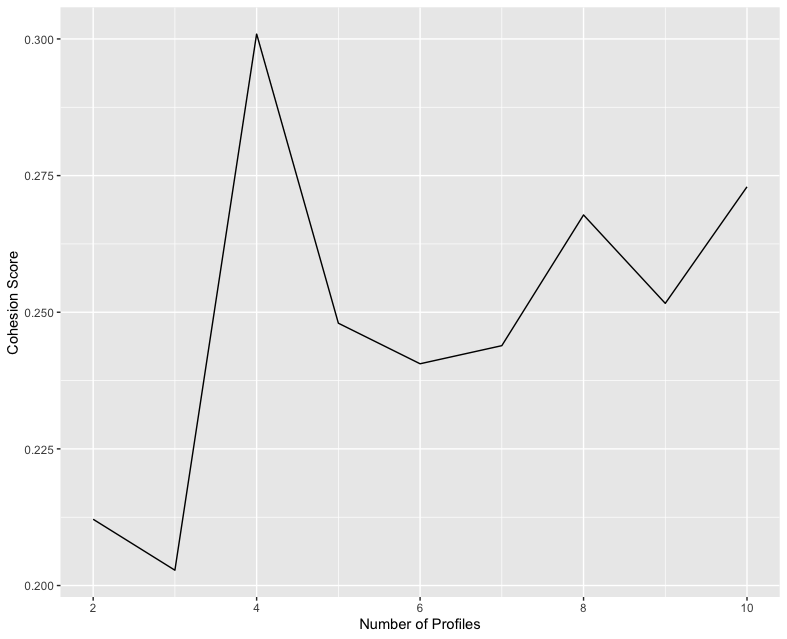
\includegraphics[width=.8\textwidth]{cohesion_score.png}
\end{center}
{\footnotesize Note: Cohesion scores for models with $M \in [\![2,10]\!]$. Topic cohesion is calculated as the average cohesion for score for features $B \in (5,10,15,20)$.}
\end{figure}


\begin{figure}[h!]
\caption{Average Cohesion from \cite{draca2020polarized}}
\begin{center}
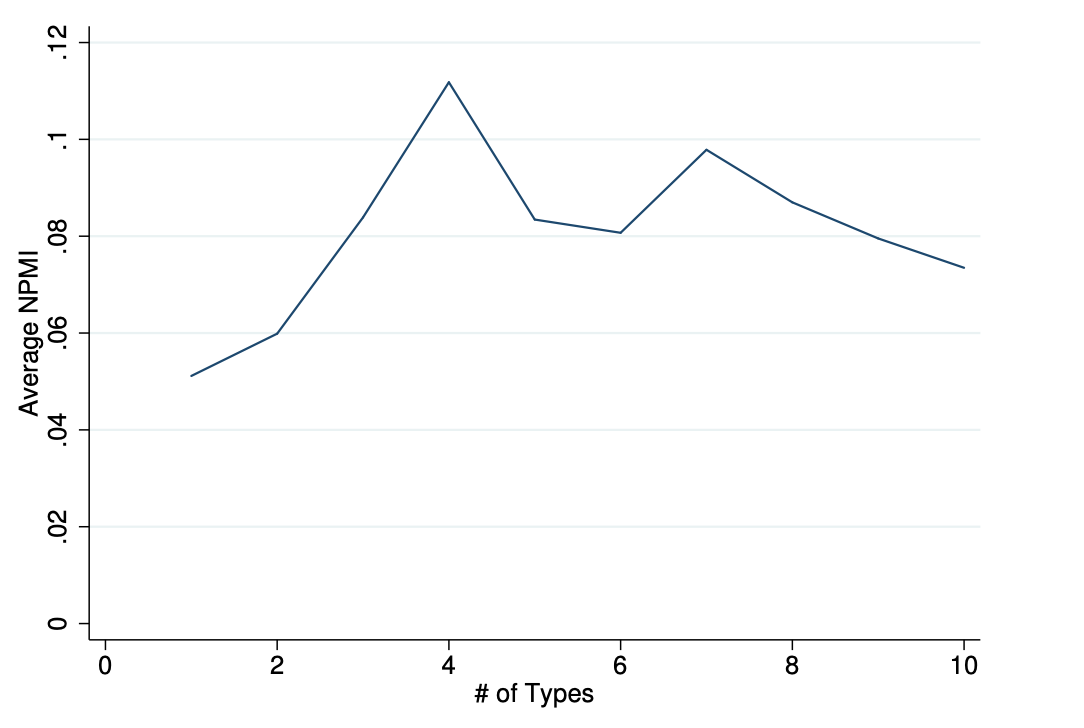
\includegraphics[width=.8\textwidth]{cohesion_score_draca_schwarz.png}
\end{center}
\end{figure}

\clearpage

\section{Regressions}
\begin{table}[h!]
    \caption{2-profiles}
    \begin{center}
        \scalebox{0.7}{\input{"topic2.tex"}}
    \end{center}
    {\footnotesize Note: The dependent variables are indicator variables equal to one if the respondent has been assigned to this profile (generally because most of her responses belong to this profile). 
    The \textit{race: White only} indicator variable equals one if the respondent's self reported race is only ``White." The regression includes controls for gender, having children and not having completed a college degree. The three \textit{status} indicator variables indicate the difference in mean compared to a reference group of people not working (either unemployed or inactive). The \textit{status: Working} indicator variable includes respondents who self-reported being either ``Full-time employed", ``Part-time employed", or ``Self-employed". The three \textit{Income} indicator variables indicate difference in mean compared to a reference group of people in the first quartile of household's annual income in 2019 (i.e. income $<$ \textdollar 35,000). The five \textit{age} indicator variables indicate difference in mean compared to a reference group of people aged between 18 and 24. The two \textit{vote} indicator variables indicate difference in mean compared to a reference group of people who either did not vote in the 2020 Presidential election or voted for another candidate than Biden or Trump.
    \newline  *p$<$0.1; **p$<$0.05; ***p$<$0.01}
\end{table} 

\begin{table}[h!]
    \caption{3-profiles}
    \begin{center}
        \scalebox{0.7}{\input{"topic3.tex"}}
    \end{center}
    {\footnotesize Note: The dependent variables are indicator variables equal to one if the respondent has been assigned to this profile (generally because most of her responses belong to this profile). 
    The \textit{race: White only} indicator variable equals one if the respondent's self reported race is only ``White." The regression includes controls for gender, having children and not having completed a college degree. The three \textit{status} indicator variables indicate the difference in mean compared to a reference group of people not working (either unemployed or inactive). The \textit{status: Working} indicator variable includes respondents who self-reported being either ``Full-time employed", ``Part-time employed", or ``Self-employed". The three \textit{Income} indicator variables indicate difference in mean compared to a reference group of people in the first quartile of household's annual income in 2019 (i.e. income $<$ \textdollar 35,000). The five \textit{age} indicator variables indicate difference in mean compared to a reference group of people aged between 18 and 24. The two \textit{vote} indicator variables indicate difference in mean compared to a reference group of people who either did not vote in the 2020 Presidential election or voted for another candidate than Biden or Trump.
    \newline  *p$<$0.1; **p$<$0.05; ***p$<$0.01}
\end{table} 

\begin{table}[h!]
    \caption{4-profiles}
    \begin{center}
        \scalebox{0.7}{\input{"topic4.tex"}}
    \end{center}
    {\footnotesize Note: The dependent variables are indicator variables equal to one if the respondent has been assigned to this profile (generally because most of her responses belong to this profile). 
    The \textit{race: White only} indicator variable equals one if the respondent's self reported race is only ``White." The regression includes controls for gender, having children and not having completed a college degree. The three \textit{status} indicator variables indicate the difference in mean compared to a reference group of people not working (either unemployed or inactive). The \textit{status: Working} indicator variable includes respondents who self-reported being either ``Full-time employed", ``Part-time employed", or ``Self-employed". The three \textit{Income} indicator variables indicate difference in mean compared to a reference group of people in the first quartile of household's annual income in 2019 (i.e. income $<$ \textdollar 35,000). The five \textit{age} indicator variables indicate difference in mean compared to a reference group of people aged between 18 and 24. The two \textit{vote} indicator variables indicate difference in mean compared to a reference group of people who either did not vote in the 2020 Presidential election or voted for another candidate than Biden or Trump.
    \newline  *p$<$0.1; **p$<$0.05; ***p$<$0.01}
\end{table} 

\clearpage

\begin{spacing}{0.5}
\bibliographystyle{chicago}
\bibliography{My_Library}
\end{spacing}
\end{document}